%=== CHAPTER THREE (3) ===
%=== (Actual work done and contribution, including literature survey) ===

\chapter{Methods}
\begin{spacing}{1.5}
\setlength{\parskip}{0.3in}
%  (Actual work done and contribution, including literature survey)
\begin{figure}[t]
    \centering
    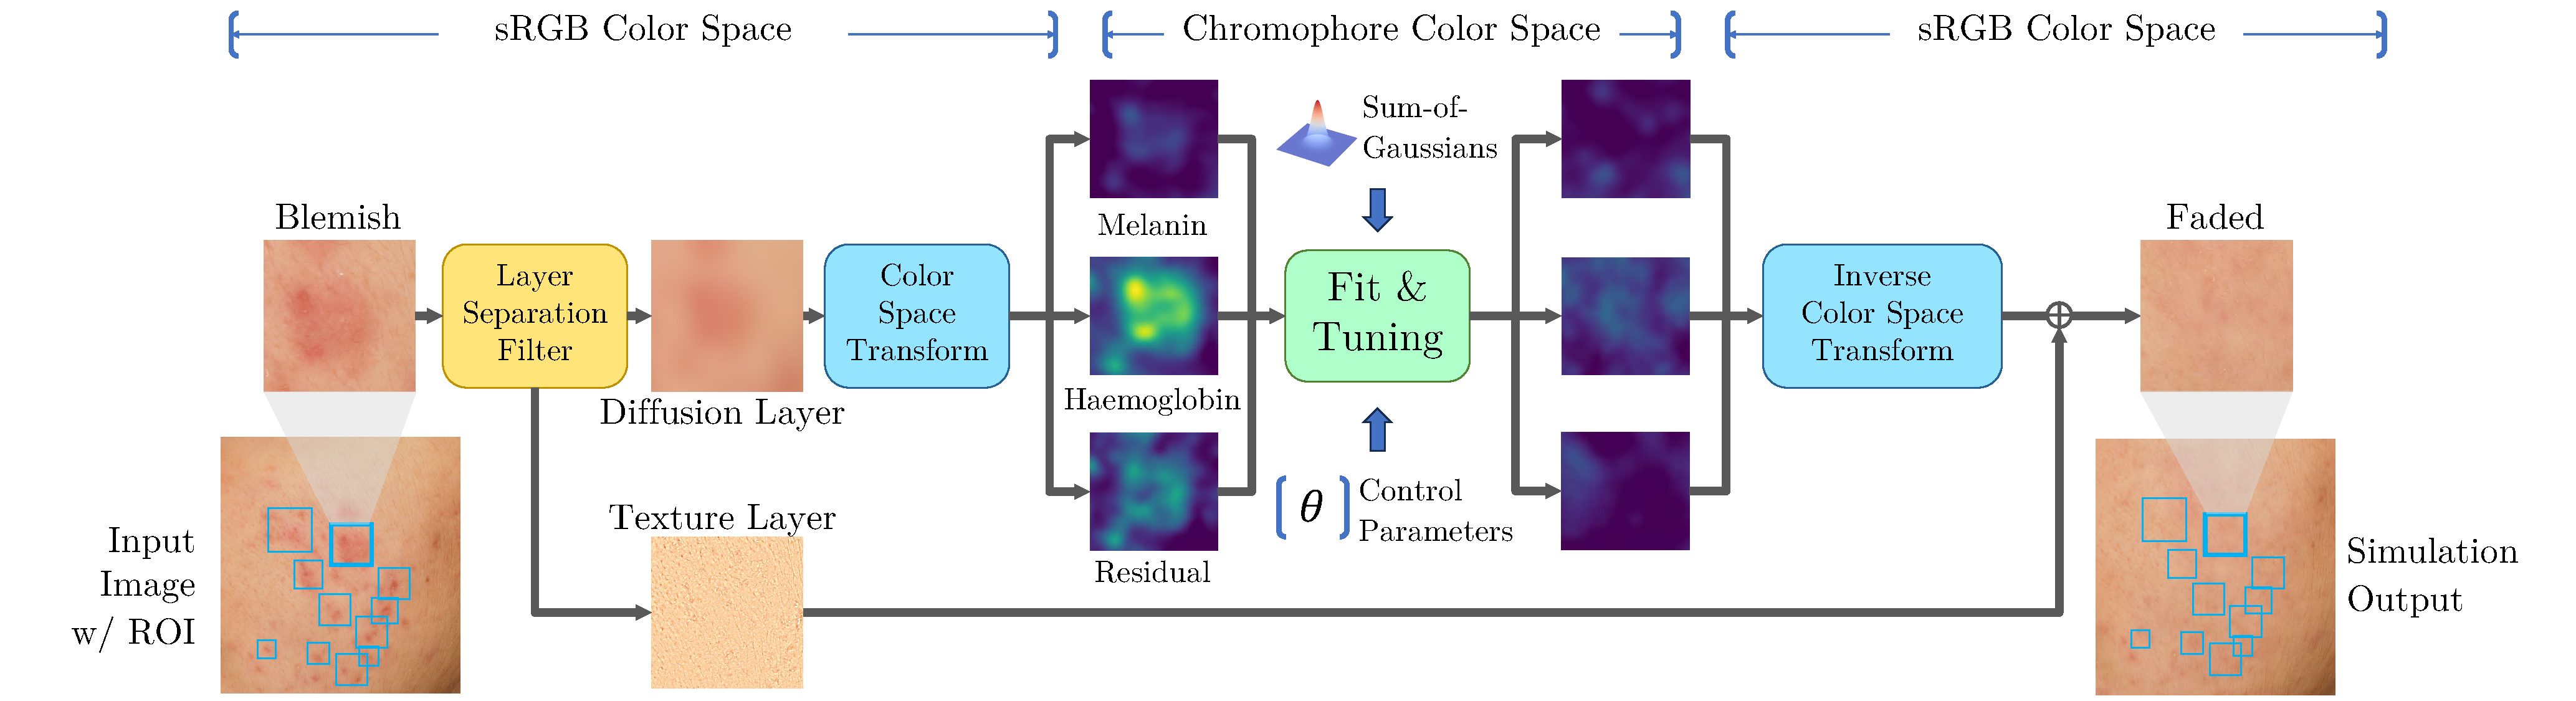
\includegraphics[width=0.94\columnwidth]{Chapter3/system.pdf}
    \caption{An overview of the proposed skin blemish change simulation pipeline. In the pipeline, a box of Region of Interest (ROI) is first used to select the blemish like acne or pigmentation. Then, a \textit{Layer Separation Filter} is applied to separate the texture layer and the diffusion layers. A \textit{Sum-of-Gaussians} model is fitted to each ROI in \textit{Melanin/Heamoglobin} color space, with the parameters of the fitted model adjusted to manipulate the appearance of the blemishes. The modified diffusion layer is summed with the original texture layer to obtain the output.}
    \label{fig:system}
\end{figure}

\section{Skin Chromophore Color Space Decomposition}
In digital photos, skin color represents only a small subset of the sRGB space, due to unique chromophores contained in the skin, such as melanin and heamoglobin, which give the skin a unique and limited color range. However, finding a transformation from sRGB values to the absolute concentration of skin chromophores is challenging, as the sRGB color space is device-agnostic. It also requires calibrating the camera system using pigmentation data in vivo. This issue is bypassed by modeling the \textit{relative} pigment concentration against the base skin, so that the transformed color space can well express the influence of different chromophores on skin color without the need for camera system calibration.

Specifically, the relative absorption of incident light by the chromophore can be described by the Beer-Lambert law, namely:
\begin{equation}
    A(\lambda) = -log(R(\lambda)) = C\epsilon l,
    \label{eq1}
\end{equation}
where $A$ represents absorption, $R$ is the reflection intensity, $\lambda$ is the wavelengths, $C$ is the relative concentration, $\epsilon$ denotes the extinction coefficient of chromophore and $l$ is the mean optical path length.

In this work, the impact of two chromophores on the skin, melanin and heamoglobin, and a residual term, are mainly considered, as shown in Figure \ref{fig:skin_model}. Therefore, $C\epsilon l$ in equation \ref{eq1} expands as
\begin{equation}
    A(\lambda) = C_H\epsilon_H(\lambda)l_H + C_M\epsilon_M(\lambda)l_M + C_r\epsilon_r(\lambda)l_r,
    \label{eq2}
\end{equation}
where subscript $H$, $M$, and $r$ represent heamoglobin, melanin, and residual chromophore, respectively.

Given the distinct absorption and reflection properties of skin chromophores under varying wavelengths of light, the response of each chromophore is considered across the three primary camera pixel channels: Red ($\mathcal{R}$), Green ($\mathcal{G}$), and Blue ($\mathcal{B}$). This consideration leads to the formulation of Equations \ref{eq1} and \ref{eq2}. These equations model the chromophore response in the context of the color channels, providing a foundation for further analysis and image processing within the scope of the proposed method.
\begin{equation}
    \begin{aligned}
         & C_H\epsilon_H^c l_H + C_M\epsilon_M^c l_M + C_r\epsilon_r^c l_r = -log(R^c) \\
         & c\in\{\mathcal{R},\mathcal{G},\mathcal{B}\},
    \end{aligned}
\end{equation}
or in matrix form
\begin{gather*}
    \mathbf{E}\mathbf{c}=-log(\mathbf{k}),\\
    \mathbf{E}=\begin{bmatrix}
        \epsilon_H^\mathcal{R} l_H & \epsilon_M^\mathcal{R} l_M & \epsilon_r^\mathcal{R} l_r \\
        \epsilon_H^\mathcal{G} l_H & \epsilon_M^\mathcal{G} l_M & \epsilon_r^\mathcal{G} l_r \\
        \epsilon_H^\mathcal{B} l_H & \epsilon_M^\mathcal{B} l_M & \epsilon_r^\mathcal{B} l_r
    \end{bmatrix},\
    \mathbf{c}=\begin{bmatrix}C_H \\C_M \\C_r\end{bmatrix},\
    \mathbf{k}=\begin{bmatrix}R^\mathcal{R} \\R^\mathcal{G} \\R^\mathcal{B}\end{bmatrix}.
\end{gather*}

It is reported that there is no significant difference in skin thickness between human races\cite{Whitmore2000}. In other words, $l$ can be seen as a constant. So $l$ is combined with $\epsilon$ in $\mathbf{E}$. Following the practice of Tsumura et al.\cite{tsumura1999independent}, $E$ is estimated by Fast Independent Component Analysis (FastICA)\cite{HYVARINEN2000411} in the log-RGB domain. Specifically, 128 patches are randomly sampled from each face skin image of the dataset, and each patch is 16x16 pixels in size. Then the average RGB value of each patch is calculated. The FastICA algorithm in \texttt{sklearn}\cite{scikit-learn} is adopted to estimate the 3 independent components over the log-RGB domain as $\mathbf{E}$. In this work, $\hat{\mathbf{E}}$ is obtained as follows:
\begin{equation}
    \hat{\mathbf{E}} = \begin{bmatrix}
        0.96  & -0.63 & 0.9  \\
        -0.22 & 0.35  & 0.17 \\
        -0.16 & -0.69 & -0.4 \\
    \end{bmatrix}
\end{equation}

\section{Spot Appearance Modelling \& Editing}
Given a 3-channel image patch $C(\mathbf{x})\in\mathbb{R}^{3\times h\times w}, \mathbf{x}\in\mathbb{R}^2$ with length $w$ and height $h$, containing a user-selected blemish, we assume it can be divided into normal skin $C_K^{skin}$ and blemish $C_K^{blem}$ in chromophore color space, that is
\begin{equation}
  C_K(\mathbf{x}) = C_K^{skin}(\mathbf{x}) + C_K^{blem}(\mathbf{x}),\quad K\in\{H,M,r\}.
\end{equation}
For the estimation of $C_K^{skin}$, we assume that skin color changes are smooth within a local area. Therefore, we fit it with a simple linear model
\begin{equation}
  \hat{C_K^{skin}}(\mathbf{x};\mathbf{k},d)=\mathbf{k}\mathbf{x}+d,\quad\mathbf{k}\in\mathbb{R}^2, d\in\mathbb{R}.
\end{equation}
For the estimation of $C_K^{blem}$, the proposed method is based on the observation that pigmentation and acne of interest tend to have blurred edges due to the subsurface scattering of light under the skin. On one hand, they are caused by local accumulation of chromophores under the skin due to various stressors such as UV or inflammation, which can be modeled as Gaussian distributions. On the other hand, subsurface scattering of light under the skin makes pigmentation look even blurry. With Gaussian functions, both phenomena can be described very well, because the convolution of two Gaussian functions is still a Gaussian function, namely:
\begin{equation}
    \begin{aligned}
         & G(x; \mu_a, \sigma_a, a)\star G(x; \mu_b, \sigma_b, b)                 \\
         & \qquad= a\cdot b\cdot G(x; \mu_a+\mu_b, \sqrt{\sigma_a^2+\sigma_b^2}),
    \end{aligned}
\end{equation}
where $\star$ is the convolution operator, and Gaussian function $G$ is defined as
\begin{equation}
    G(x; \mu, \sigma, a) = \frac{a}{\sigma\sqrt{2\pi}}e^{-\frac{{(x - \mu)^2}}{{2\sigma^2}}}.
\end{equation}
For multivariate Gaussian functions (2D in this research), they can be denoted as
\begin{equation}
    G(\mathbf{x}; a, \mathbf{\mu}, \Sigma)=\frac{a}{2\pi\sqrt{|\Sigma|}}e^{-\frac{1}{2}(\mathbf{x}-\mathbf{\mu})^T\Sigma^{-1}(\mathbf{x}-\mathbf{\mu})},
  \end{equation}
where $\mathbf{\mu}=[\mu_x,\mu_y]^T$ is the centre coordinate $(x,y)$ on the input image plane, $\Sigma\in\mathbb{R}^{2\times2}$ is the covariance matrix and $a$ is the amplitude factor. And note that the above conclusion can also be generalized to this multivariate case.

To better fit variously shaped blemishes and uneven facial areas, $\Sigma$ can be further decomposed into multiplication of rotation matrix $\mathbf{R}$ and scaling matrix $\mathbf{S}$ as
\begin{equation}
    \Sigma= \mathbf{R}\mathbf{S}\mathbf{S}^T\mathbf{R}^T.
\end{equation}
This allows Gaussian functions to stretch and off-axis rotation with an angle of $\theta\in[0,\pi)$, forming ellipsoidal patterns, that is
\begin{equation}
  \mathbf{R} = \begin{bmatrix}
    \cos\theta & -\sin\theta \\
    \sin\theta & \cos\theta
  \end{bmatrix},\quad\mathbf{S}=diag(\sigma_x,\sigma_y).
\end{equation}
Or explicitly
\begin{equation}
    \begin{aligned}
         & G(x, y; \mu_x, \mu_y, \sigma_x, \sigma_y, \theta, a)\\
         & \qquad=\frac{a}{2\pi \sigma_x \sigma_y}\cdot e^{-\frac{{x''^2}}{{2 \sigma_x^2}} - \frac{{y''^2}}{{2 \sigma_y^2}}},\ where \\
         & x'=x - \mu_x, \quad y'=y - \mu_y, \\
         & x'' = x' \cos\theta - y' \sin\theta,\quad y'' = x' \sin\theta + y' \cos\theta.
    \end{aligned}
\end{equation}
Finally, following the existing fast subsurface scattering implementations, the appearance of a blemish under the scattering skin tissue is approximated by sum of multiple Gaussian functions. That is, the estimated distribution $\hat{C_K^{blem}}(\mathbf{x})$ can be denoted by
\begin{equation}
  % \begin{aligned}
  \hat{C_K^{blem}}(\mathbf{x}; \Theta)=\sum_{i=0}^{N-1}G_i(\mathbf{x}; \Theta_i),\ N\ge1, \Theta_i=\left[a_i, \mathbf{S}_i, \mathbf{\mu}_i, \theta_i\right].
  % \end{aligned}
\end{equation}
The parameters are fitted by the Levenberg-Marquardt method\cite{10.1007/BFb0067700} with the \texttt{lmfit} Python library\cite{newville_matthew_2014_11813}. After successful fitting, $\hat{C_K^{skin}}$ is discarded. Instead, $\hat{C_K^{blem}}$ is multiplied with a user-input gain $\alpha_K\in\mathbb{R}$ and add it with the input $C_K(\mathbf{x})$ to amplify/attenuate the blemish intensity to obtain the modified image patch $C_K^{\prime}$, namely
\begin{equation}
  C_K^{\prime} = C_K+\alpha_K\hat{C_K^{blem}}.
  \label{eqn:alpha}
\end{equation}
Obviously, if $\alpha_K=-1$, the facial blemish will be completely removed from the image patch, while a positive gain will intensify this blemish.

\subsection{Algorithm Implementations}
\subsubsection{Preporcessing}
% As shown in Figure \ref{fig:system}, in the pipeline, a skin layer separation filter is first adopted to separate the skin into a surface texture layer (including specular reflections and skin textures) and a scattered chromophore layer. This is implemented using a Gaussian filter with a small variance, small enough to isolate the detail texture of the skin without affecting the underlying assumptions.
In the proposed methodology, as depicted in Figure \ref{fig:system}, the primary focus is laid on the \textit{Diffusion Layer} of the image. To isolate this layer, a skin layer separation filter is first adopted to separate the skin into a surface \textit{Texture Layer} (including specular reflections and skin textures) and a \textit{Diffusion Layer}. This is implemented using a Gaussian filter with a small variance, small enough to isolate the detail texture of the skin without affecting the underlying assumptions. 

Subsequently, in color space transform stage, inverse gamma correction is applied to the standard RGB (sRGB) image to derive linear RGB values. These values are then converted to their logarithmic form, representing an approximation of the real reflectance values, denoted as $R$ in Equation\ref{eq1}. While this approximation may not perfectly mirror the actual scenario, it proves adequate for estimating the relative concentration ratio in comparison to the surrounding skin.
\subsubsection{Optimizations in Fitting Process}
In the actual implementation, several optimizations are performed to the program:
\begin{itemize}
    \item Each channel and each spot can be fitted independently and multi-process parallelism can be used to speed this up. Thus, the program packages each fitting session into a task and uses Python's thread pool to build a task queue, fully utilizing the computing power of multi-core CPUs.  
    \item Although the entire Sum-of-Gaussians model could be fitted at once, the convergence of the fit would be slow. Therefore, a strategy is adopted where a new $N$-th Gaussian function is gradually introduced into the model with $N-1$ functions and the updated model is fitted, during which the existing parameters are frozen. Finally, all parameters are unfrozen for one more fitting as a fine-tuning. In this way, only one function is fitted each time except for the last one.
    \item In Levenberg-Marquardt iterations, it requires compute the Jacobian matrix for each steps. Since each component in $\hat{C_k}$ has explicit partial derivatives and they are just simply summed togeter, the Jacobian matrix of $\hat{C_k}$ can be manually derived. This assists the Levenberg-Marquardt algorithm to quickly compute accurate gradients rather than estimate them numerically.
\end{itemize}
This algorithm can be represented by the following pseudocode.
\begin{algorithm}
    \caption{Fitting Distribution of a Spot}
    \begin{algorithmic}[1]
    
    \State \textbf{Input:} Spot image patch $X\in\mathbb{R}^{3\times h \times w}$, per-channel gain $\alpha_K\in\mathbb{R}^3$. All from user-input.
    
    \State \textbf{Preprocessing:}
    % \Indent
        \State $X_d, X_t \gets GaussianFilter(X)$ \Comment{$X_d$:Diffusion Layer, $X_t$:Texture Layer}
        \State $X_d \gets \gamma^{-1}(X_d/255.0)$ \Comment{Inverse gamma transformation to linear RGB space}
        \State $X_d \gets \mathbf{E}^{-1}\cdot\log{X_d}$ \Comment{Transform to chromophore color space}
    \For{each channel $k \in \{H, M, r\}$ of $X_d$}
        \State Initialize linear normal skin model $\hat{C_k}\gets\hat{C_k^{skin}}$
        \For{each Gaussian component $G^i_k$}
            % \State Estimate initial center position $x^{init}_i, y^{init}_i$
            \State Fit $G_k^i(x, y; \mu_x^i, \mu_y^i, \sigma_x^i, \sigma_y^i, \theta^i, a^i)$
            \State $\hat{C_k} \gets \hat{C_k}+G_k^i$
            \State Freeze parameters of $\hat{C_k}$
        \EndFor
        \State Unfreeze all parameters for final refinement fit
        \State $\hat{C_k} \gets \alpha_k\cdot(\hat{C_k}-\hat{C_k^{skin}})$
    \EndFor
    \State $X_d \gets X_d+\hat{C_k}$
    \State $X_d \gets InverseColorTransform(X_d)$
    \State $X \gets X_d+X_t$
    \State \textbf{Return:} Fitted parameters and modified spot image
    \end{algorithmic}
    \end{algorithm}
\subsubsection{GUI Implementations}
\begin{figure}[t!]
    \centering
    % \begin{subfigure}{.95\textwidth}
    %     \centering
    %     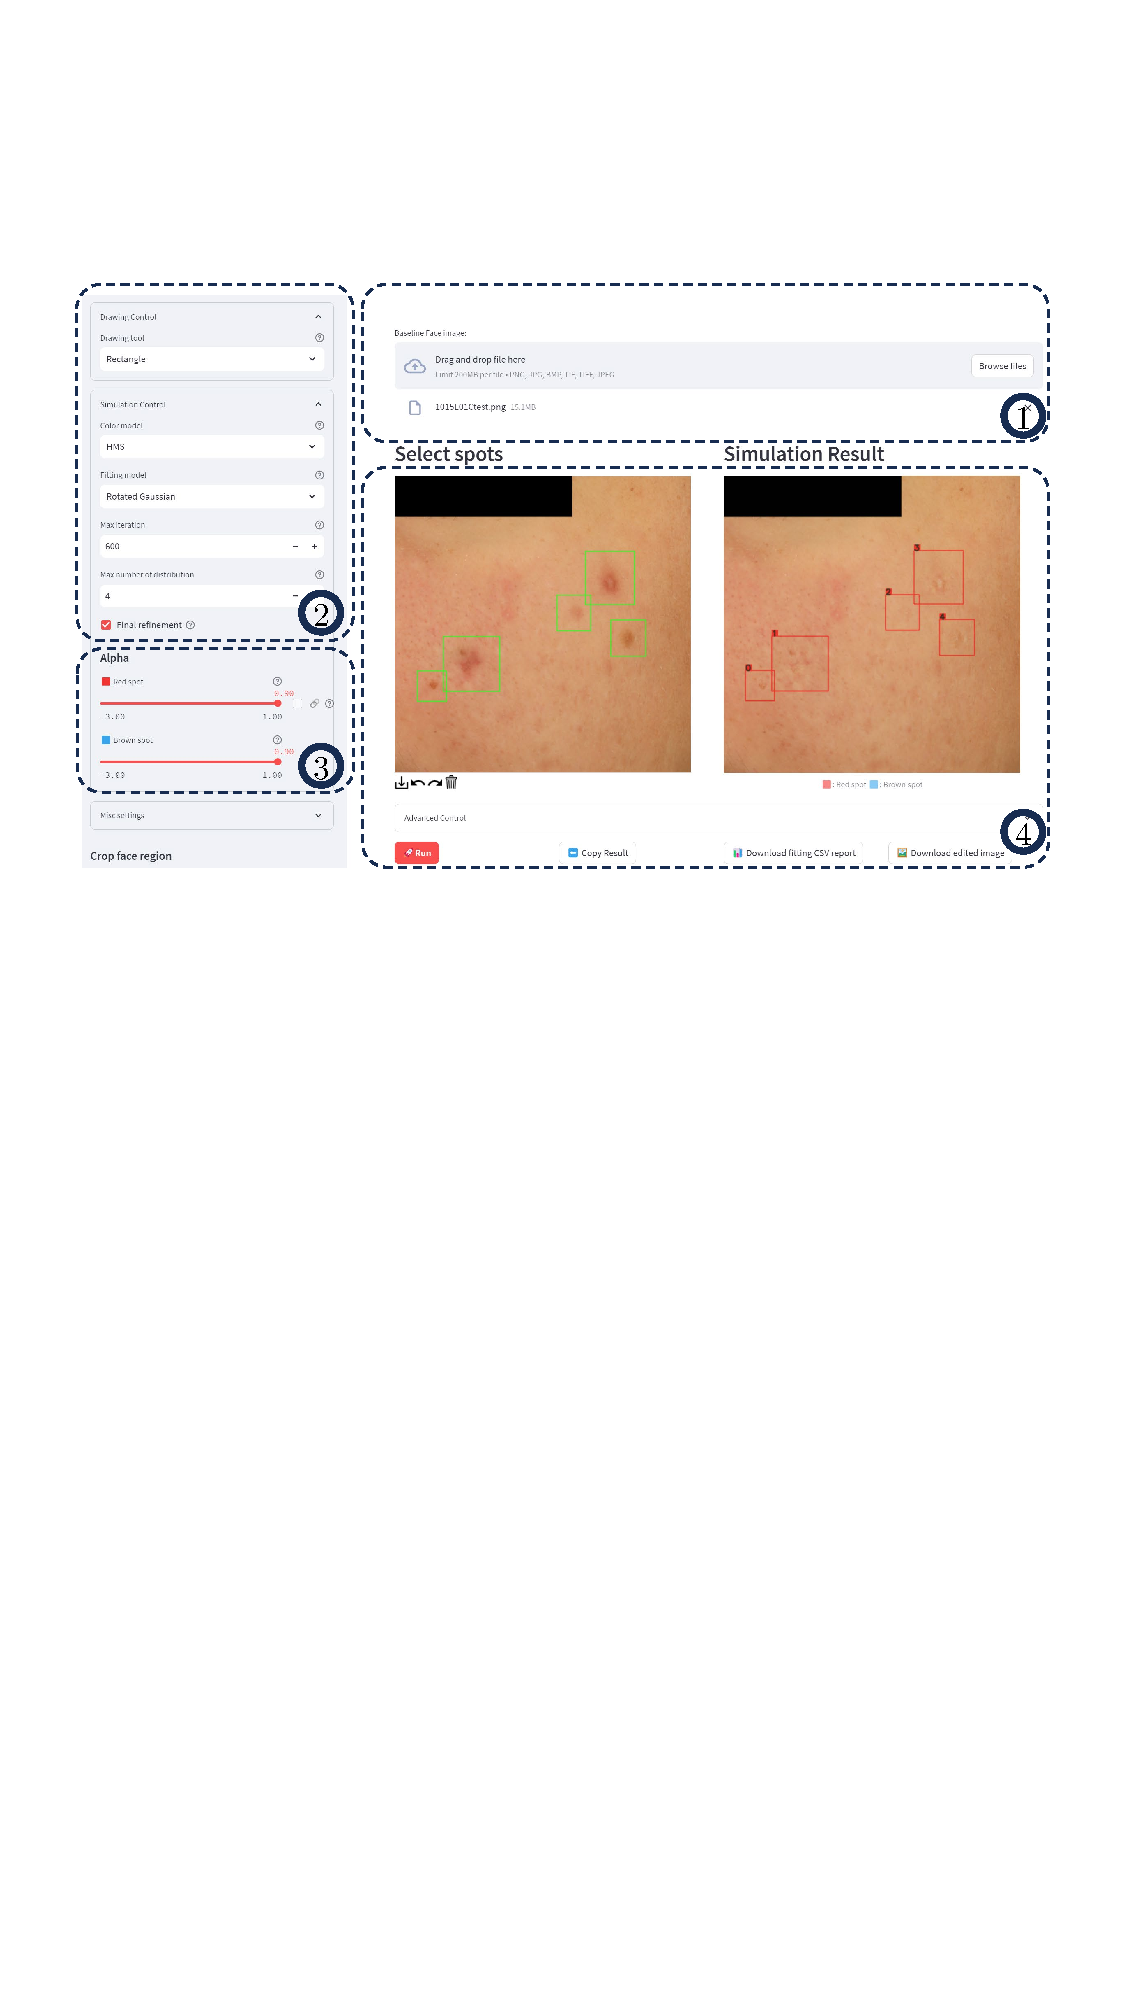
\includegraphics[width=0.95\columnwidth]{Chapter3/GUI1.pdf}
    %     % \caption{Use}
    %     % \label{fig:gui1}
    % \end{subfigure}\hfill
    % \begin{subfigure}{.95\textwidth}
    %     \centering
    %     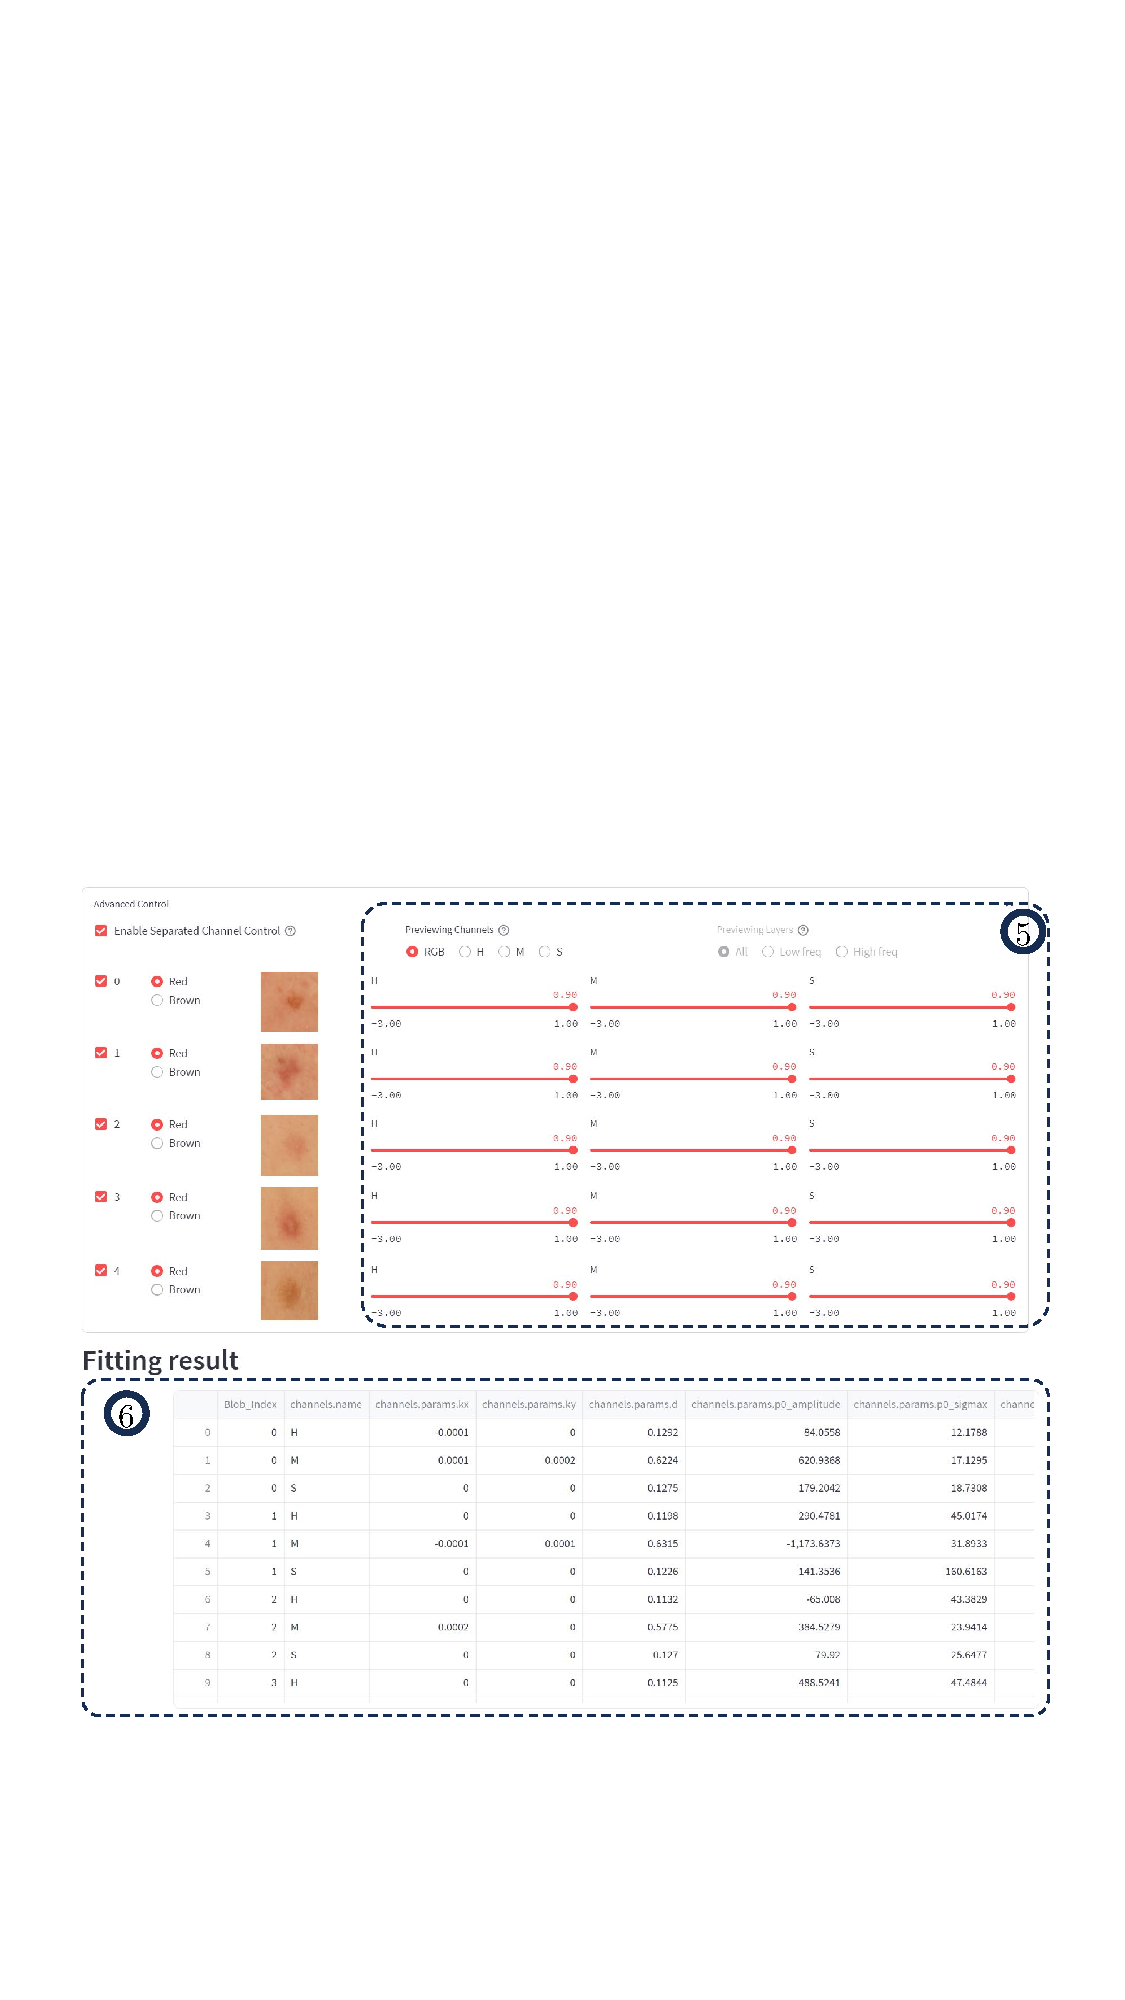
\includegraphics[width=0.95\columnwidth]{Chapter3/GUI2.pdf}
    %     % \caption{Bar chart of survey results}
    % \end{subfigure}
    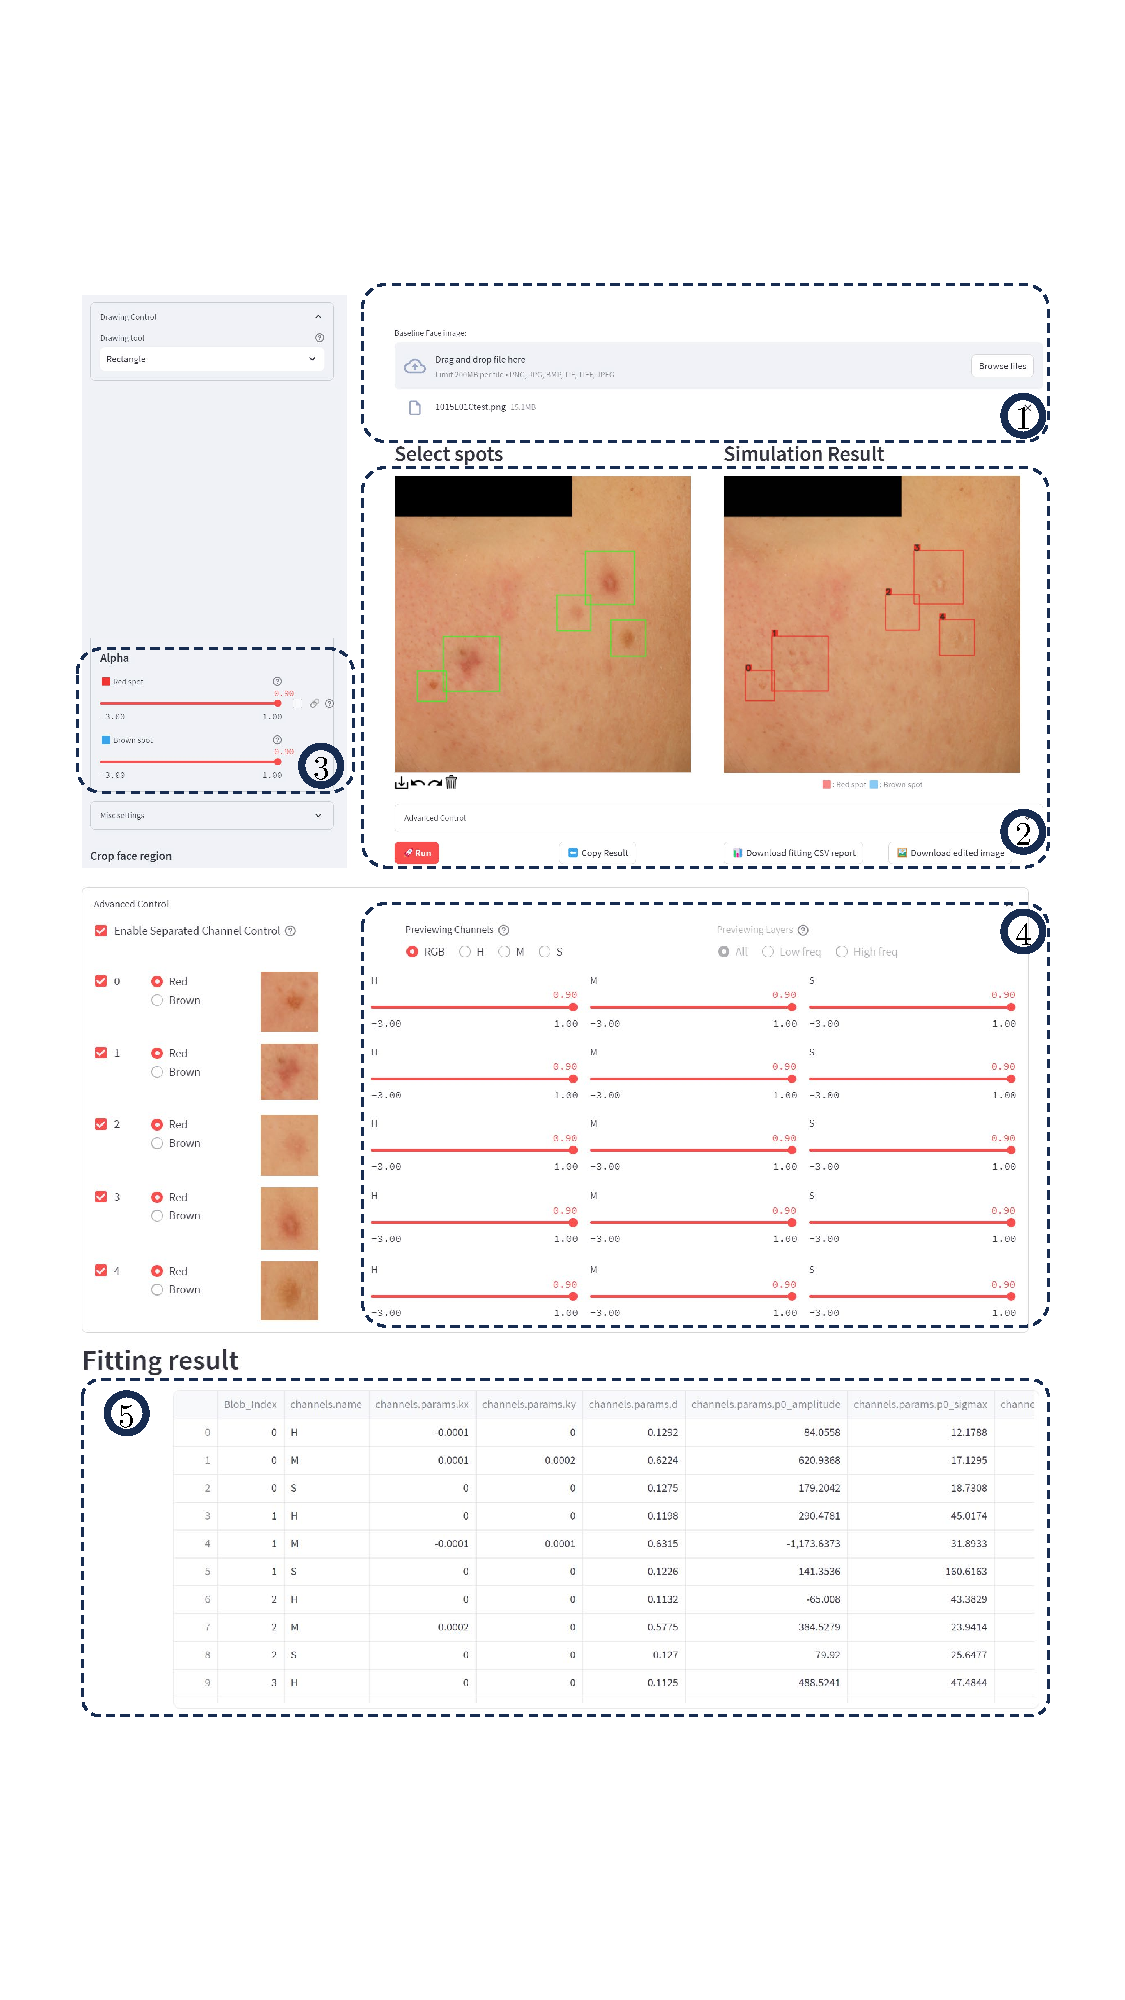
\includegraphics[width=0.9\columnwidth]{Chapter3/GUI.pdf}
    \caption{An Overview of GUI}
    \label{fig:gui}
\end{figure}
A simple graphical user interface (GUI) is also created to facilitate the editing of facial images by users with varying levels of expertise. The GUI is organized into several sections, each providing tools for specific tasks in the editing process.
\begin{itemize}
    \item \textbf{Image Upload and Spot Selection} The initial interaction with the interface is the image upload functionality, denoted by circled numeral 1 in Figure \ref{fig:gui}. Users can upload the facial image they intend to edit. Following the upload, the image is displayed within the central work area of the GUI, allowing users to identify and select skin spots for removal or modification. This selection process is designed to be intuitive, employing a simple point-and-click mechanism to mark areas of interest, as indicated by circled numeral 2.
    \item \textbf{Basic and Advanced Editing Controls} Post spot selection, users can adjust the editing intensity using the 'alpha' parameter, a slider control located in the section marked by circled numeral 3. This allows for the manipulation of the editing gain in a user-friendly manner. Activating the 'Run' button initiates the rendering process, culminating in the display of the modified image where the selected spots have been processed according to the specified parameters.

    For users requiring more sophisticated control, the interface offers advanced editing options as shown in circled numeral 4. This advanced control panel permits individual adjustments to the gains of separate color channels, thus affording an enhanced level of precision in the spot editing process.
    \item \textbf{Parameter Exportation for Analysis} An essential feature of the GUI, highlighted in circled numeral 5, is the ability to download the fitting results. This function caters to expert users who wish to perform a detailed analysis of the editing parameters or to utilize these parameters for further processing steps, thereby extending the capabilities of the system.
\end{itemize}
%=== END OF CHAPTER THREE ===
\end{spacing}
\newpage
